\documentclass{article}
\usepackage[a4paper, total={6in, 8in}]{geometry}
\usepackage[utf8]{inputenc}
\usepackage{tikz}
\usepackage{amsmath}

\usetikzlibrary{calc,patterns,angles,quotes}



\title{The Simple Pendulum, Revisted}
\author{Instructor: Jason Ho}
\begin{document}

\maketitle
\section*{Objectives}
\begin{itemize}
    \item To numerically solve the nonlinear ordinary differential equation for the simple pendulum and compare against previously collected experimental data.
    \item To explore numerical methods for solving ordinary differential equations using a variety of computational tools.
    \item To examine, analyze, and explain a sample of Python code.
\end{itemize}
\section{Introduction}
\begin{figure}
\centering
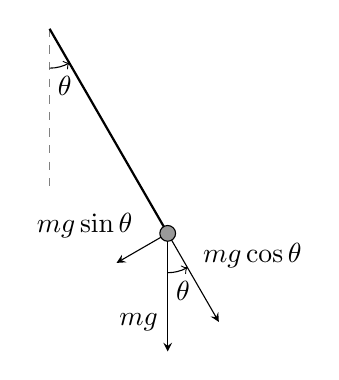
\begin{tikzpicture}
    % save length of g-vector and theta to macros
    \pgfmathsetmacro{\Gvec}{1.5}
    \pgfmathsetmacro{\myAngle}{30}
    % calculate lengths of vector components
    \pgfmathsetmacro{\Gcos}{\Gvec*cos(\myAngle)}
    \pgfmathsetmacro{\Gsin}{\Gvec*sin(\myAngle)}

    \coordinate (centro) at (0,0);
    \draw[dashed,gray,-] (centro) -- ++ (0,-2.0) node (mary) [black,below]{$ $};
    \draw[thick] (centro) -- ++(270+\myAngle:3) coordinate (bob);
    \pic [draw, ->, "$\theta$", angle eccentricity=1.5] {angle = mary--centro--bob};
    %\draw [blue,-stealth] (bob) -- ($(bob)!\Gcos cm!(centro)$);
    \draw [-stealth] (bob) -- ($(bob)!-\Gcos cm!(centro)$)
      coordinate (gcos)
      node[midway,above right] {$mg\cos\theta$};
    \draw [-stealth] (bob) -- ($(bob)!\Gsin cm!90:(centro)$)
      coordinate (gsin)
      node[midway,above left] {$mg\sin\theta$};
    \draw [-stealth] (bob) -- ++(0,-\Gvec)
      coordinate (g)
      node[near end,left] {$mg$};
    \pic [draw, ->, "$\theta$", angle eccentricity=1.5] {angle = g--bob--gcos};
    \filldraw [fill=black!40,draw=black] (bob) circle[radius=0.1];
\end{tikzpicture}
\label{fig:pendulum}
\caption{Schematic for a simple pendulum of mass $m$.}
\end{figure}
\subsection{Theory}
By looking at the total torque on a simple pendulum system (Figure \ref{fig:pendulum}) associated with the tangential direction of motion, we can derived an equation from Newton's II Law for rotations describing the (time-dependent) angular acceleration $\alpha(t)$ of a pendulum bob of mass $m$
\begin{equation}
    \alpha = \frac{\sum_i \tau_i}{m L^2},
\end{equation}
where $L$ is the distance from the axis of rotation to the center of mass of the bob. When fully simplified, we're left with an equation for $\alpha(t)$ depending on constants such as the length of the pendulum, the acceleration due to gravity, and the variable $\theta(t)$. We leave deriving this equation as a later exercise for the student, but since $\alpha(t)$ may be related to the angular coordinate $\theta (t)$ via the kinematic relationship
\begin{equation}
    \alpha(t) = \frac{d^2\theta(t)}{dt^2},
\end{equation}
we can write our equation for $\alpha(t)$ as a second-order non-linear ordinary differential equation in terms of $\theta(t)$. 

In a previous lab, in order to solve this difficult differential equation, we introduced the \textit{small-angle approximation}. For small values of the angle $\theta(t)$, using a Taylor series expansion defined by
\begin{equation}
    f(\theta) = \sum_{n=0}^{\infty} \frac{1}{n!}\left(\theta-a\right)^n\frac{d^n}{d\theta^n}f(a)
\end{equation}
where $\frac{d^n}{d\theta^n}f(a)$ is the $n^\mathrm{th}$ derivative of $f$ evaluated at $\theta= a $, we can expand our trigonometric functions about a value of $a = 0$ to find
\begin{gather}
    \cos\theta = 1 - \frac{1}{2}\theta^2+\ldots\\
    \sin\theta = \theta - \frac{1}{3} \theta^3 + \ldots\\
    \tan\theta = 1 + \frac{1}{3} \theta^3 + \ldots
\end{gather}
By truncating these series at leading order, we can approximate for values of $\theta$ close to zero that
\begin{gather}
    \cos\theta \approx 1 \\
    \sin\theta \approx \theta \\
    \tan\theta \approx 1 .
\end{gather}
This is the small-angle approximation we took previously to simplify the second-order non-linear ordinary differential equation we previously found, giving us a differential equation of the form
\begin{equation}
    \frac{d^2\theta(t)}{dt^2} = -\frac{g}{L} \theta,
\end{equation}
which gives us the solutions of a simple harmonic oscillator,
\begin{equation}
    \theta(t) = \theta_0 \cos\left(2\pi\sqrt{\frac{L}{g} }\,\,t\right),
\end{equation}
where $\theta_0$ represents the initial angle of release of the pendulum. 

For this lab, we \textit{will not} take the small-angle approximation, but instead use a method to try and find a numerical solution to the second-order non-linear ordinary differential equation found from Newton's II Law for rotations. Although we won't be able to find a nice tidy equation for our solution, we will be able to solve the system to as precise a value as we want to calculate. Along the way, we'll discover the limitations of numerical methods, and how they might be overcome. 
\section{Materials}
\begin{itemize}
    \item Microsoft Excel
    \item Python template
    \item Data from previous lab (\textit{The Simple Pendulum})
\end{itemize}
\section{Procedure}
\begin{enumerate}
    \item Starting from Newton’s II Law for rotational systems and a free-body diagram, work out an expression for the angular acceleration $\alpha$ of a simple pendulum in terms of the angle $\theta$ measured from the pendulum’s equilibrium position. Rewrite the expression you found in terms of an ordinary differential equation (ODE) of $\theta(t)$. Since this is a differential equation with a second-order derivative, we classify it as a \textit{second-order ordinary differential equation}.
    \item \textbf{Thinking about relationships between kinematic variables,} discuss with your table how we might rewrite this second-order ODE as two first-order ODE (\textit{i.e.}, as two equations with only first-order derivatives). Once you think you have the two equations, check-in with a TA to check your work.
    \item How could you approximate your equations using what you know about derivatives and calculus? (\textit{Hint:} how do we define a derivative? How do we think about a derivative in the context of graphing a function?) Here, we’re making an approximation, just like we did previously with the small angle approximation. What’s different about this approximation?\footnote{The formula you should arrive at is called \textbf{Euler’s Method}. There are more sophisticated ways to solve ODEs numerically, but this is one of the simplest.}
    \item Using Excel, numerically solve the ODE without the small angle approximation using Euler’s Method. 
    \begin{enumerate}
        \item In a blank spreadsheet, define the following constants: acceleration due to gravity $g = 9.81\,\mathrm{m/s^2}$, pendulum length $L = 1\,\mathrm{m}$, timestep $\Delta t = 0.1 \,\mathrm{s}$, initial angle $\theta_0 = \pi/18$, and initial angular speed $\omega_0 = 0\,\mathrm{s^{-1}}$.
        \item Plot $\alpha(t)$ vs. $t$, $\omega(t)$ vs. $t$, and $\theta(t)$ vs. $t$ (on the same graph, if you'd like). First, check to see if you’ve coded everything in correctly. What do you expect the behavior of each function to look like? What are the initial values supposed to be? Where should the maximum and minimum values be? Where should the zero values be? Do you see any problems with your graph?
        \item Now, extend your plotting range out to $t=30 \,\mathrm{s}$. What do you notice? 
        \item Finally, check to see what happens if we look at larger initial angles. Set $\theta_0 = \pi/3$ and replot out to $t = 30\,\mathrm{s}$. What happens to your graph?
        \item If anything unusual happened in your graphs above, what could be the cause of it? 
    \end{enumerate}
    \item Using Python, numerically solve the ODE without the small angle approximation using Euler’s Method. 
    \begin{enumerate}
        \item Open your web browser and go to\href{}{}. We’ll be looking at Python code using a Jupyter notebook environment which will allow us to run code in blocks. We will use Docker to run the Jupyter notebook through a web browser instead of configuring the software on each individual computer. 
        \item Familiarize yourself with the code by answering the following questions with your table.
        \begin{itemize}
            \item What Python variables correspond to the variables you used in Excel?
            \item What equations are the same? How are they different?
            \item Is the variable corresponding with $\theta$ coded in degrees, or radians?
            \item What does the function \verb!alpha(x)! do? How is it different from what you defined in Excel?
            \item There are two other numerical methods programmed into the template other than Euler’s method: the Midpoint method, and Verlet’s method. How are they different than Euler’s method? How are they the same?
        \end{itemize}
        \item Modify the function \verb!alpha(x)! so that it matches the expression you derived and used in the Excel sheet. If you need to assign a variable a value, add a line in the function that follows \verb!variable = number!. For now, just assign a value of $L = 1\,\mathrm{m}$ for the length of the pendulum. 
        \item In your own words, describe what the function is doing when you run the following lines of code:
        \footnotesize
        \begin{verbatim}
        time=ODESolver(omega_0 = 0, theta_0 = 45, delta_t=0.1, n_iter=300).euler(alpha).time_
        theta=ODESolver(omega_0 = 0, theta_0 = 45, delta_t=0.1, n_iter=300).euler(alpha).theta_    
        \end{verbatim}
        \normalsize
        (be specific as possible!)
        \item Using the same values as in your Excel activity, plot out the angle of oscillation as a function of time for 30 seconds. On a rough glance, how does your plot compare to the one you found in Excel?
        \item Let’s remember that in solving this ODE numerically, we’re making an assumption. In Excel, it’s a little annoying to play with this assumption, but in Python it’s pretty easy. Strengthen your assumption made in creating this numerical model and replot your graph from the previous step (making sure you’re still plotting the graph over 30 seconds). What changed?
    \end{enumerate}
    \item Compare your large-$\theta$ results from the previous lab to the predictions from one of the numerical models built in this lab. 
    \begin{enumerate}
        \item Choose three values period measurements from your last lab, including at least one with an initial angle larger than $30^\circ$. Inputting the correct pendulum length, and using the Python template, determine the predicted period from the model using Euler’s method. How does the model compare to your measurements? 
    \end{enumerate}
\end{enumerate}
\textit{\textbf{Stretch goal:}} What does the analysis look like if you use the other methods programmed into \verb!ODESolver()!? Is there a method that works better, and why? 




\end{document}
